\chapter{The Daya Bay Reactor Antineutrino Experiment}
\label{ch:detector}

The Daya Bay Reactor Antineutrino Experiment was designed
to be sensitive to $\thetaot \sim 0.01$
by performing a relative measurement of the rate of \nuebar{}
using a modular detector system arranged at near and far sites \cite{dybproposal2006}.
The experiment is located in southeast China,
approximately \SI{55}{\km} northeast of Hong Kong,
on the campus of the Daya Bay and Ling Ao Nuclear Power Plants.
Data taking began on 24 December 2011 and is planned to continue
until December 2020.

The Daya Bay site is ideal for an oscillation experiment.
Its six reactor cores together form one of the most intense \nuebar{}
sources on Earth \cite{dybproposal2006}.
The power plant campus is also located at the base of a mountain ridge,
providing an ideal location for antineutrino detectors that need to be
protected from cosmic-ray muons without having to dig deep mines.
The tunnel layout allows for easy access to the experiment via electric golf cart.

\section{Reactors and experimental halls}

Six pressurized-water nuclear reactor cores are used
as the \nuebar{} source for Daya Bay.
Each reactor has an output of \SI{2.9}{\giga\watt_{th}}
and combined they produce approximately \num{3.5e21}\,\nuebar/s \cite{ngd2016}.
The reactors are arranged in three pairs: Daya Bay, Ling Ao, and Ling Ao II.
The location of the cores determined the layout of the Daya Bay experiment.

The experiment is arranged into three experimental halls (EHs).
EH1 is located close to the Daya Bay cores (\SIrange{350}{400}{\meter}),
and EH2 is located close to the Ling Ao and Ling Ao II cores
(\SIrange{450}{550}{\meter}).
They are therefore known collectively as the near halls.
Their purpose is to constrain the \nuebar{} flux for the
relative oscillation measurement,
and they each contain two antineutrino detector modules (ADs).
EH3 is located farther away, approximately \SI{2}{\km} from the Daya Bay cores
and \SI{1.5}{\km} from the Ling Ao cores,
and is correspondingly also called the far hall.
EH3 is located at the first oscillation minimum
for the oscillation controlled by \thetaot,
and its purpose is to measure the decrease in \nuebar{} rate compared to the near halls.
To increase statistics, EH3 contains four ADs.
The layout of the EHs with respect to the reactors is shown in \cref{fig:layout}.

\begin{figure}
    \centering
    \begin{subfigure}{0.49\textwidth}
        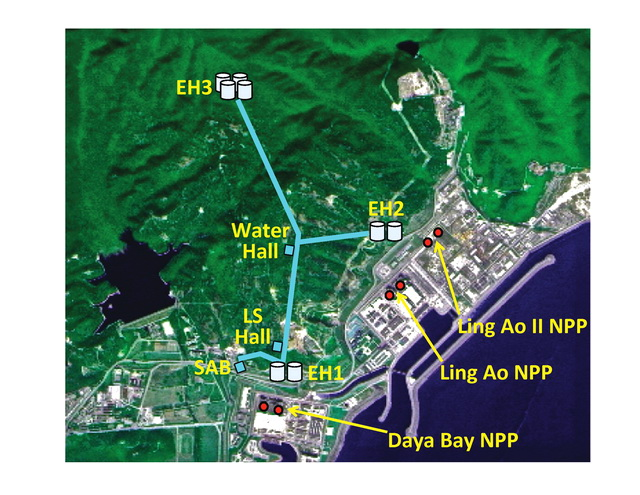
\includegraphics[width=\textwidth]{ch_detector/dayabay_map}
    \end{subfigure}
    \begin{subfigure}{0.49\textwidth}
        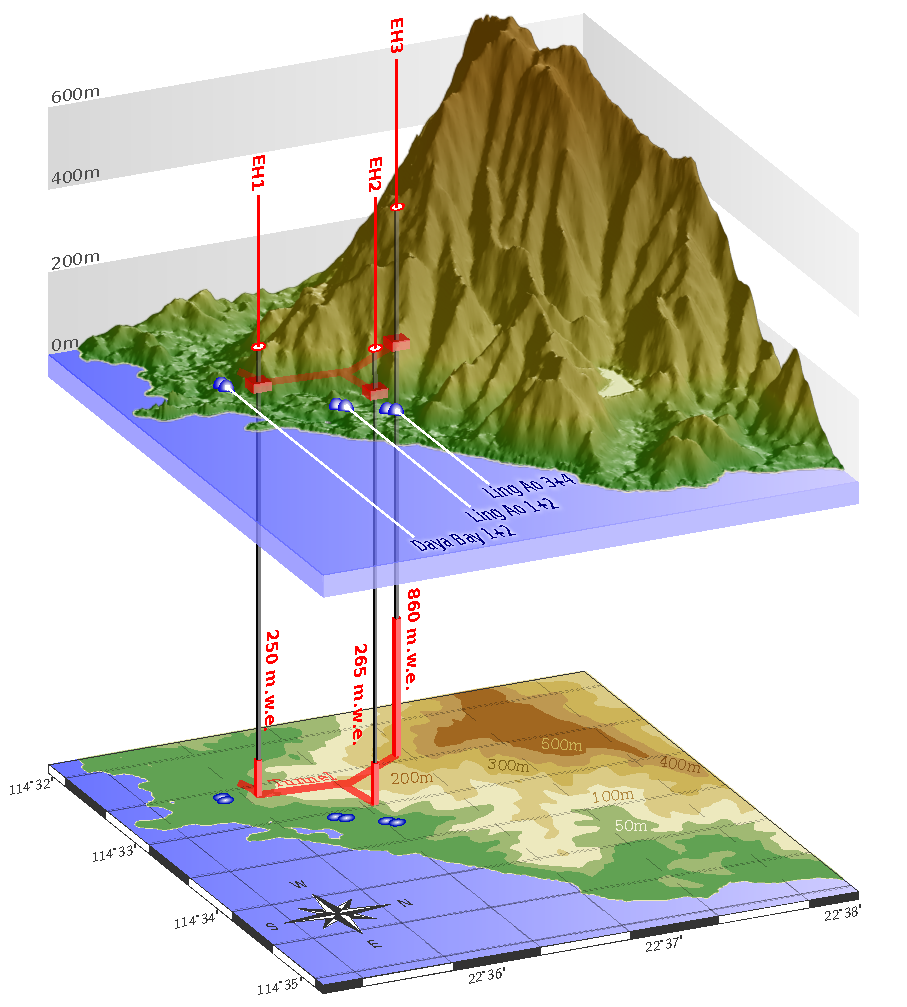
\includegraphics[width=\textwidth]{ch_detector/dayabay_map_3d}
    \end{subfigure}
    \caption{Two views of the layout of the Daya Bay experiment.}
    \label{fig:layout}
\end{figure}

The EHs are located at underneath a mountain, which provides a substantial
overburden to protect against cosmic-ray muons.
The specific measurements of overburden, the positions of the ADs,
and the baseline are shown in \cref{tab:baselines}.

\begin{figure}
    \missingfigure{Table of baselines and overburdens}
    \label{tab:baselines}
\end{figure}

To accelerate the experiment startup timeline,
only six of the planned eight ADs were installed in 2011:
2 in EH1, 1 in EH2, and 3 in EH3.
This so-called 6-AD period lasted from December 2011 until July 2012.
The experiment was shut down while the remaining two ADs were installed
in EH2 and EH3.
The 8-AD period began in October 2012.
At the end of 2017, EH1-AD1 was chosen to be repurposed as a test stand
for liquid scintillator studies for the JUNO experiment \cite{junoproposal2016},
and was decommissioned from Daya Bay.
The 7-AD period began in January 2017 and will continue through the end of
the Daya Bay experiment in December 2020.

The ADs within each hall are collectively surrounded by a water pool,
which acts as a passive shield against natural radioactivity present in the rock
as well as an active veto for muons which penetrate through the overburden.
The water pool is covered by a resistive plate chamber (RPC) array
to provide additional sensitivity to incoming muons.
\Cref{fig:eh3_wp_photo} shows a photograph of EH3 during installation of the ADs,
when the RPC had not yet been moved into position to cover the water pool.
Also visible mounted to the near and far walls are two muon telescopes
which were used for muon studies during detector commissioning \cite{muonsystem2015}.

\begin{figure}
    \centering
    \includegraphics[width=0.5\textwidth]{ch_detector/EH3_installation_6ADperiod}
    \caption{EH3 during the installation of the first three ADs.}
    \label{fig:eh3_wp_photo}
\end{figure}

\section{Antineutrino detectors}

The eight antineutrino detectors (ADs) are used to measure
the rate and energy of millions of \nuebar interactions with high precision
and low systematic uncertainty.
Each AD consists of three concentric cylindrical regions
contained in an outer stainless steel vessel (SSV),
a cylinder with diameter and height of \SI{5}{\m}.
The innermost region is filled with \SI{0.1}{\percent} by mass
Gadolinium-doped liquid scintillator (GdLS).
The GdLS is contained within an acrylic cylinder known as the inner acrylic vessel (IAV).
The middle region between the IAV and the outer acrylic vessel (OAV) is filled
with (plain, undoped) liquid scintillator (LS).
The outer region between the OAV and SSV is filled with mineral oil
that serves as a final passive layer of shielding around the LS region.

Two views of the nested AD configuration are shown in \cref{fig:ad_cutaway}.
The IAV has a height and diameter of \SI{3}{\m} and is filled with \SI{20}{\tonne}
of GdLS.
The OAV has a height and diameter of \SI{4}{\m} and is filled with \SI{20}{\tonne}
of LS.
The SSV has a height and diameter of \SI{5}{\m} and is filled with \SI{40}{\tonne}
of mineral oil.
Each acrylic vessel is made of UV-transparent acrylic
and has a thickness of approximately \SI{1.5}{\cm}.
The liquid scintillator is linear alkylbenzene.
\todo{Describe LAB}
Each AD contains overflow tanks to allow the liquid in each region
to respond to the slight expected changes in temperature and pressure.
ADs were also fitted with three automated calibration units (ACUs)
which contain radioactive sources and LEDs to help calibrate the ADs.
The ACUs are described in detail in \cref{ch:calibration}.

The mineral oil region also contained the 192 8-inch Hamamatsu R5912
photomultiplier tubes (PMTs) that monitor the AD for scintillation light
(and, secondarily, Cherenkov radiation).
The PMTs are arranged in 8 rings of 24 PMTs on the outer edge of the mineral oil region.
Light collection and detector uniformity is increased by the presence of
specular reflectors located on the top and bottom faces of the OAV,
as indicated in \cref{fig:ad_cutaway}.

\begin{figure}
    \centering
    \begin{subfigure}{\textwidth}
        \centering
        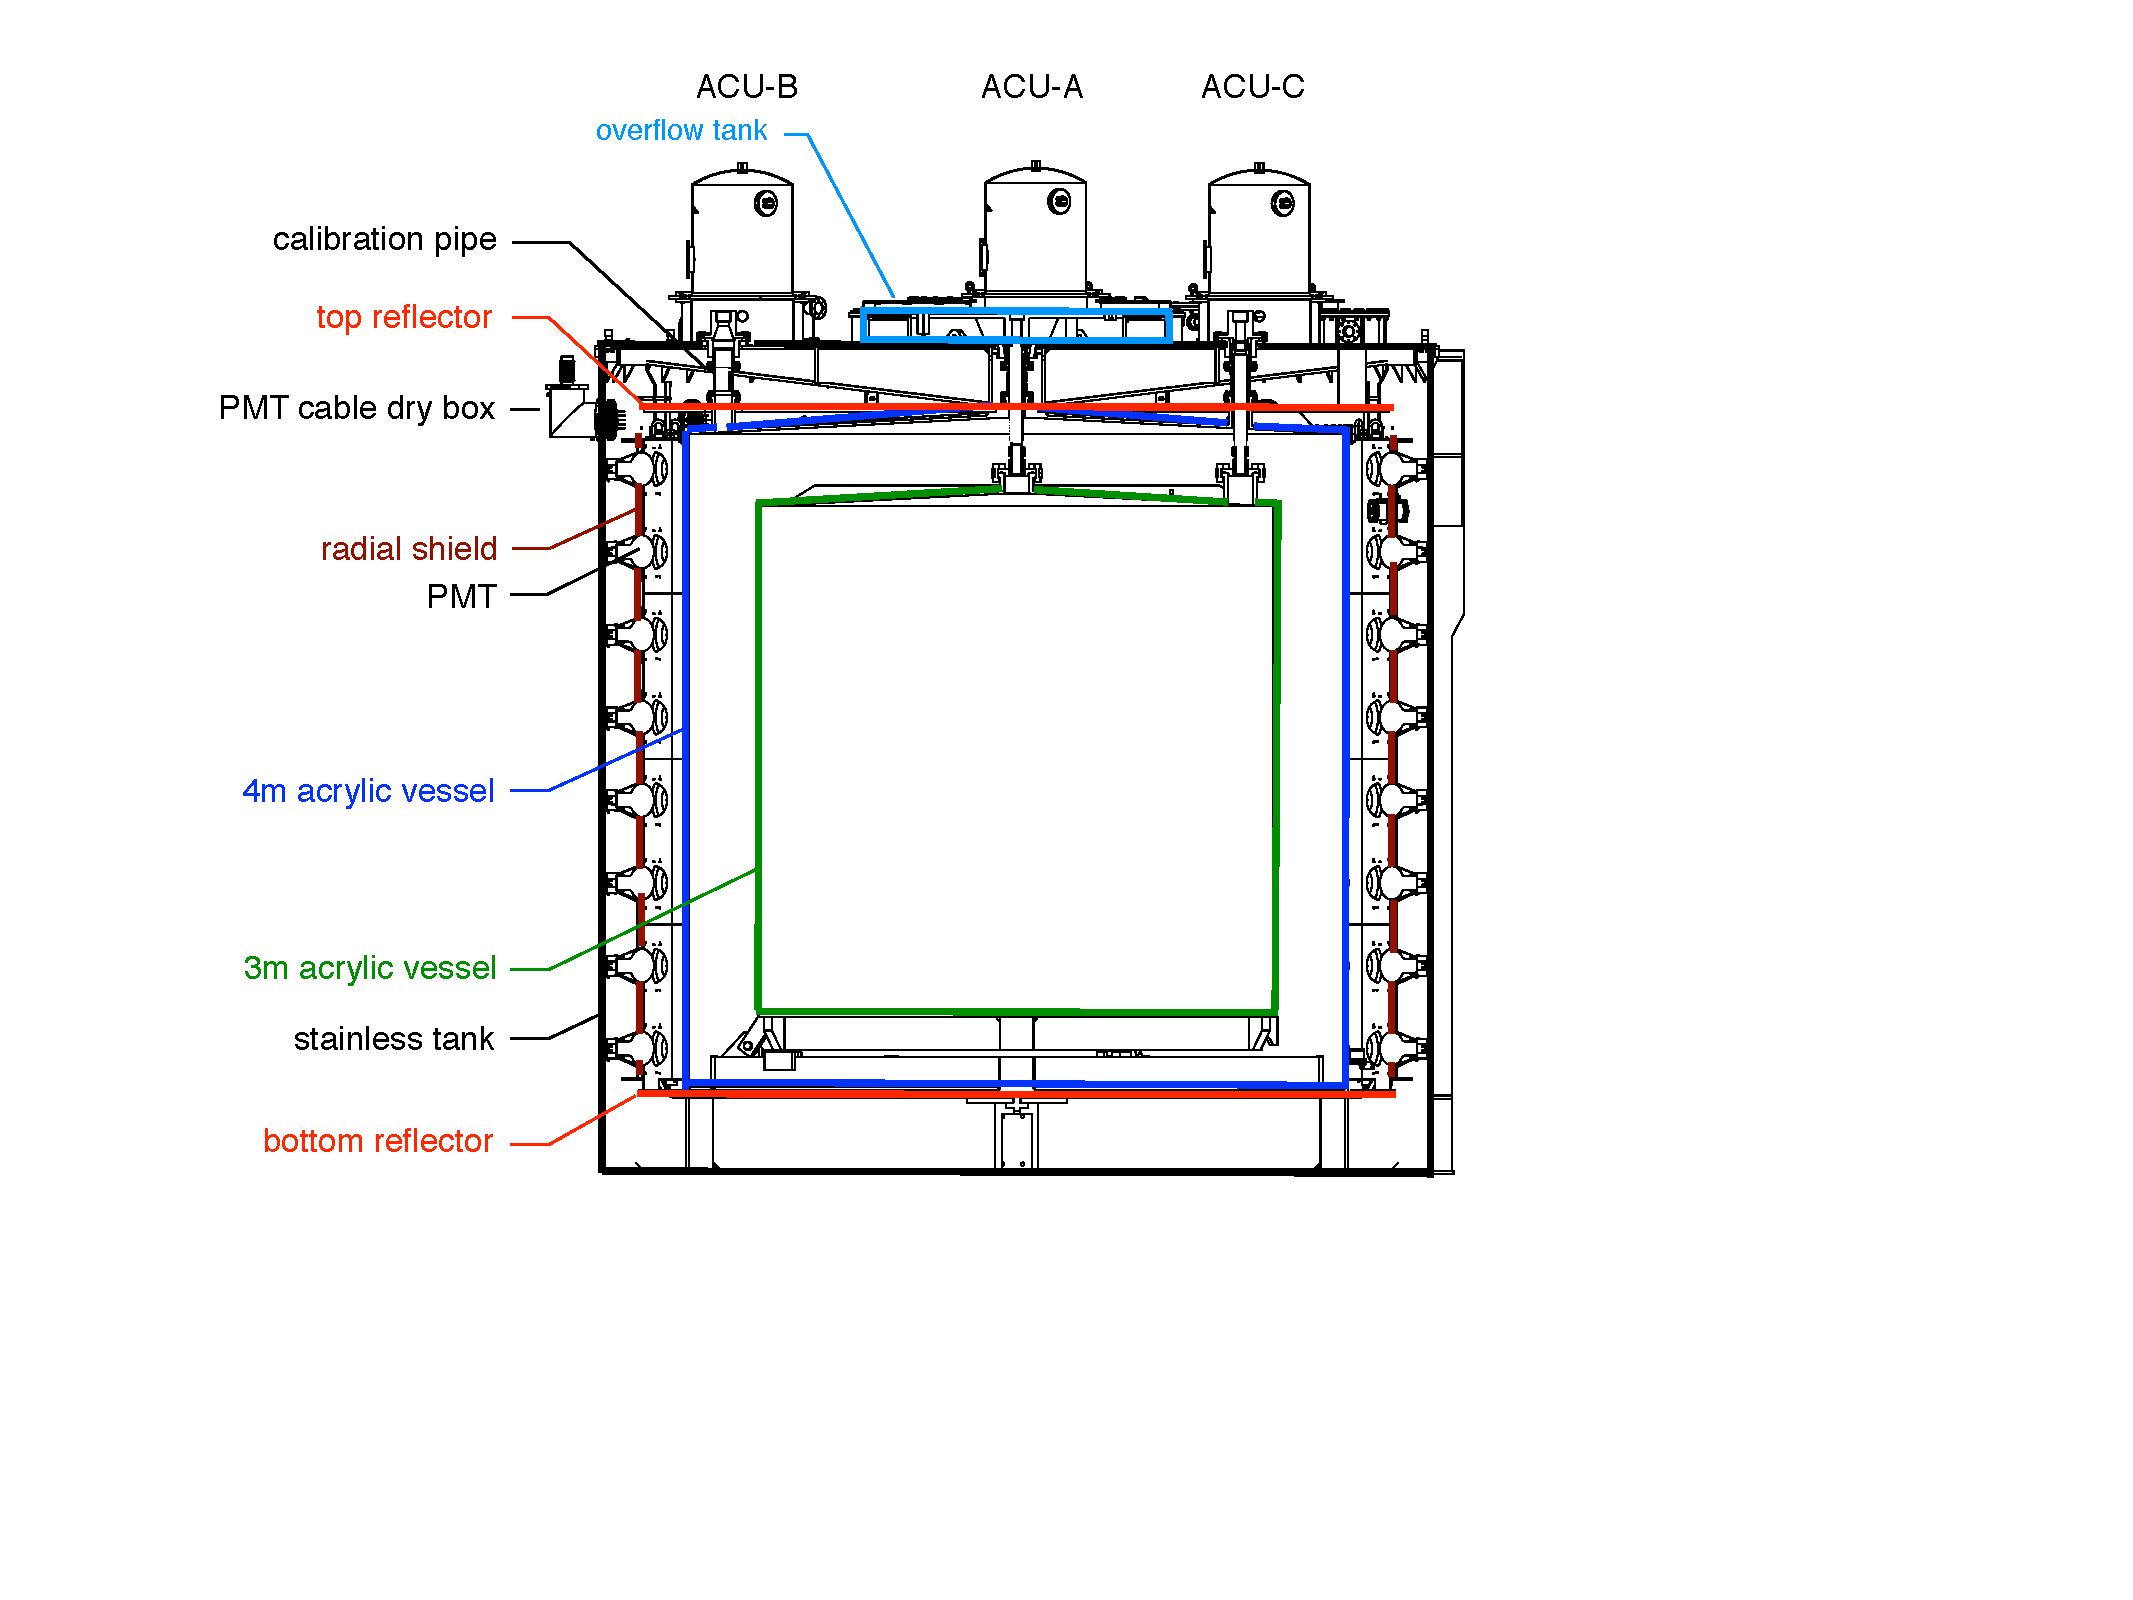
\includegraphics[height=0.4\textheight]{ch_detector/ADcutaway_2D}
    \end{subfigure}
    \vspace{1cm}\\
    \begin{subfigure}[0.4\textheight]{\textwidth}
        \centering
        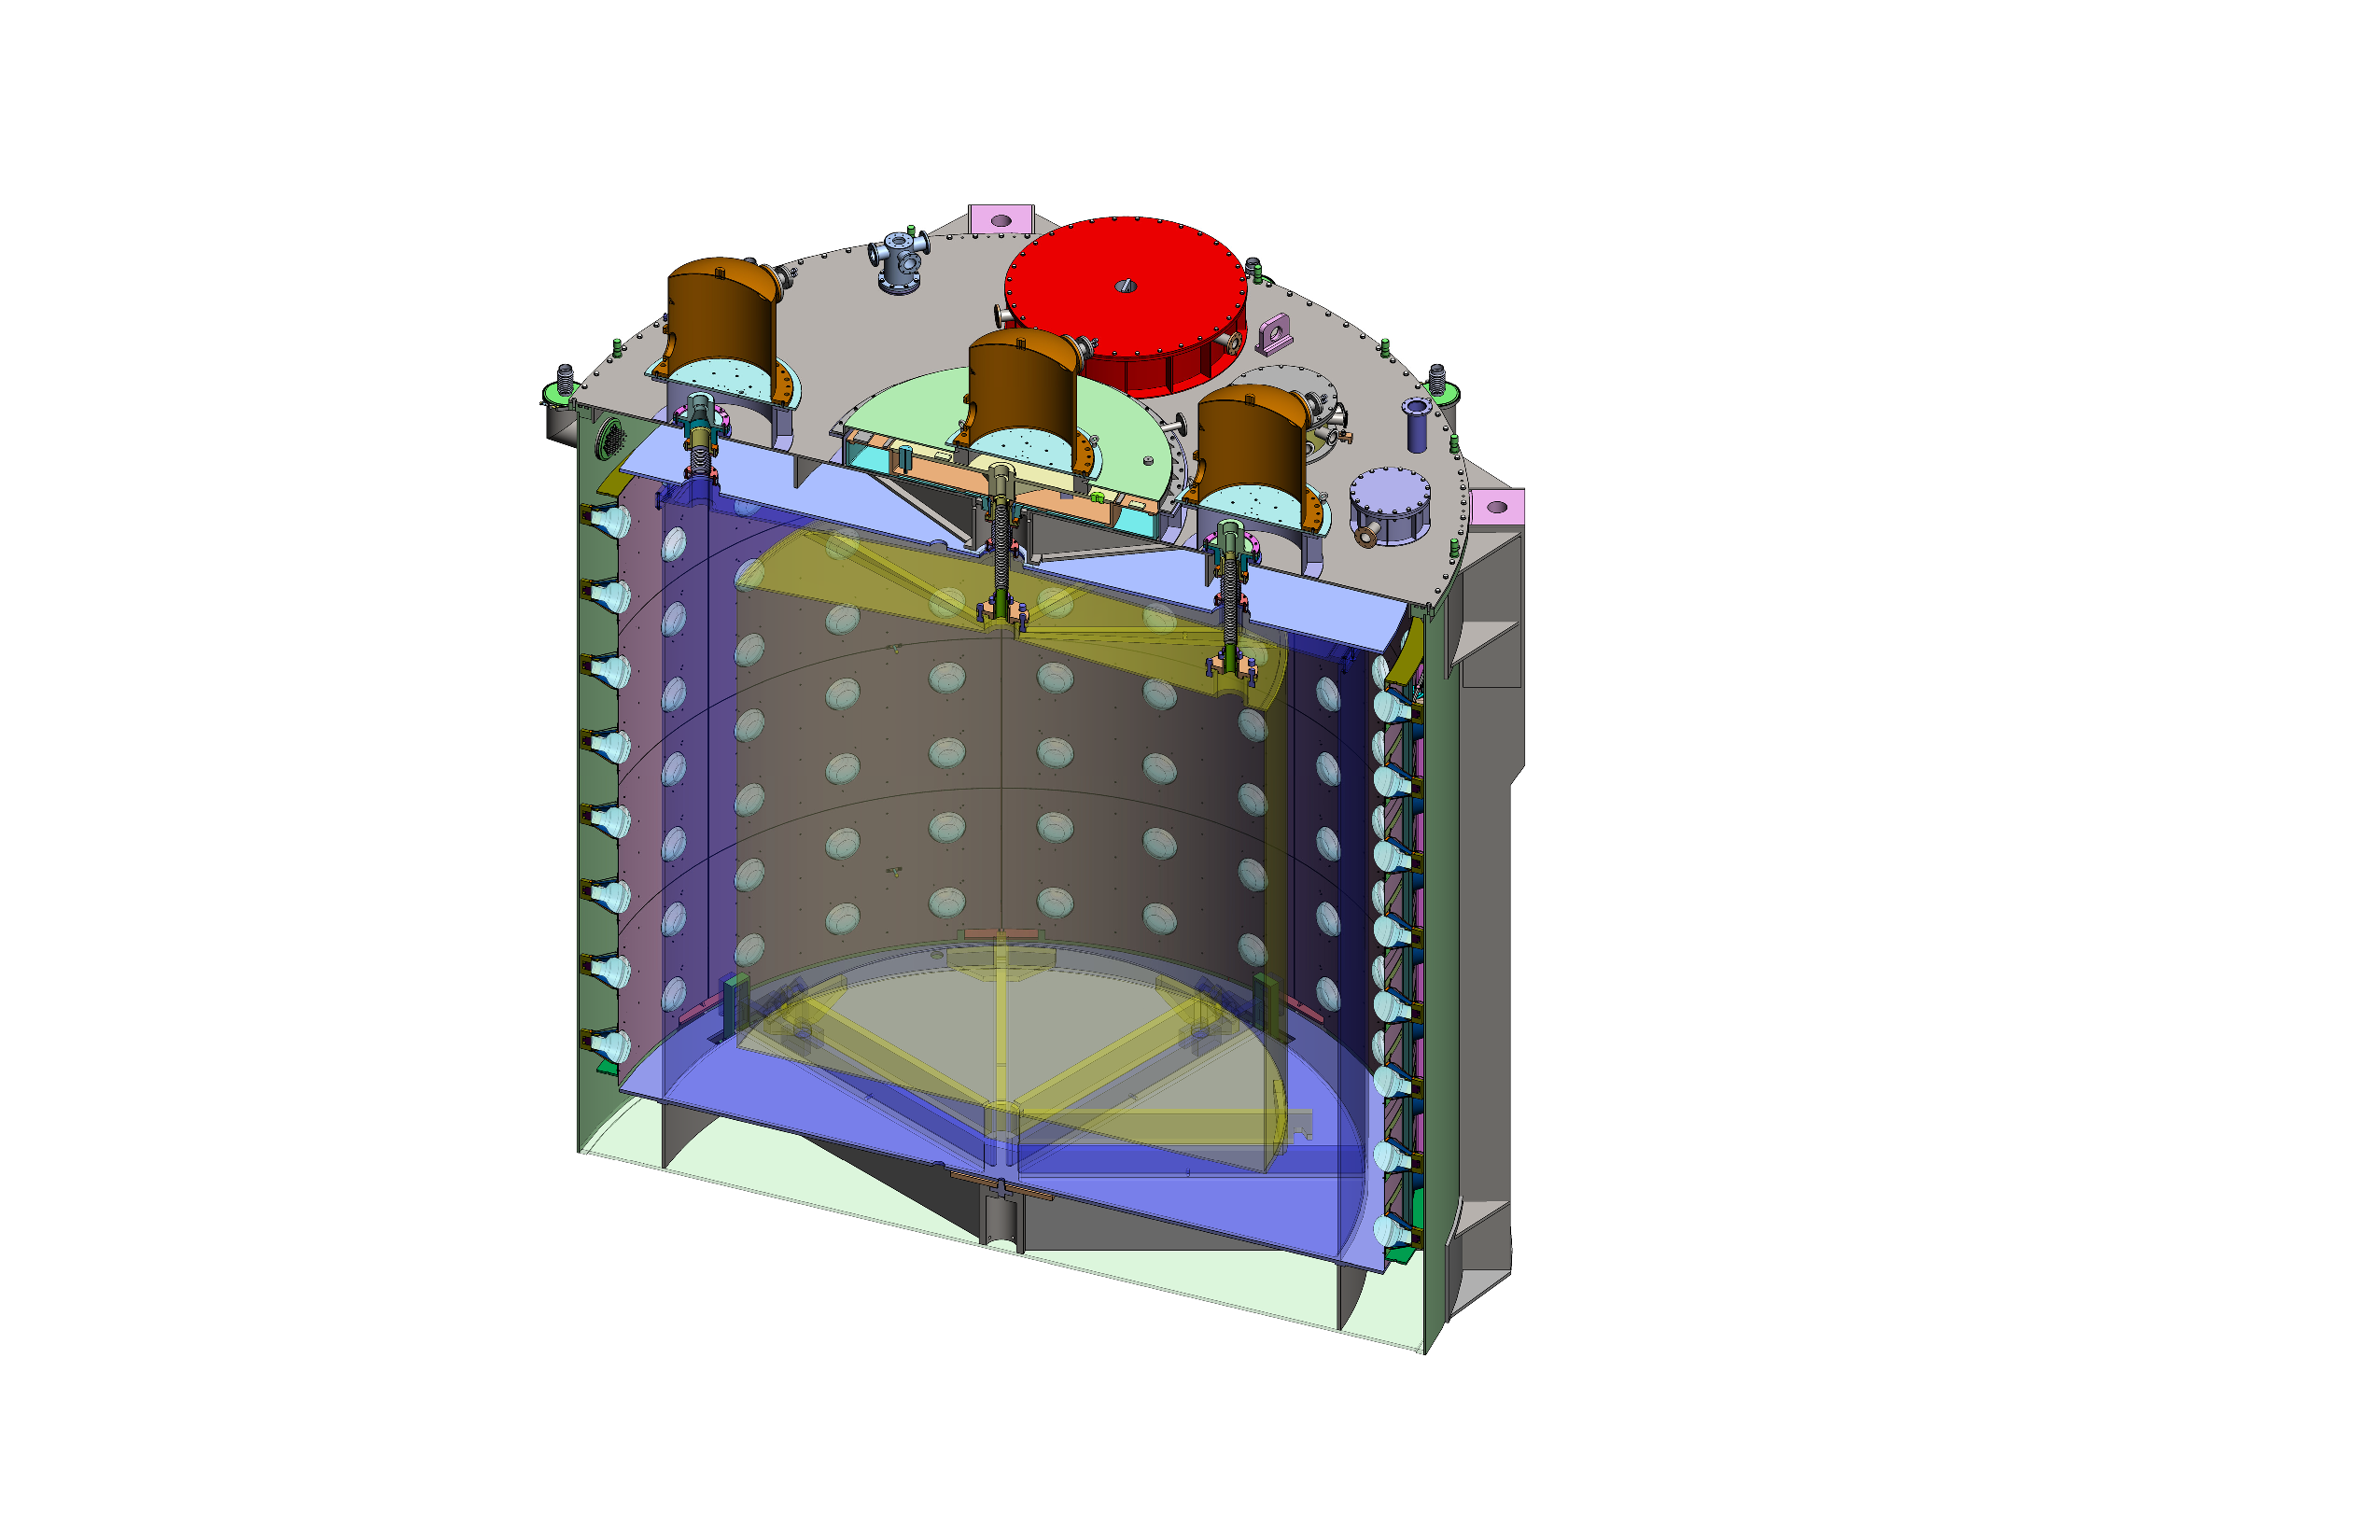
\includegraphics[height=0.4\textheight]{ch_detector/ADcutaway}
    \end{subfigure}
    \caption{Two views of the Daya Bay antineutrino detector (AD)}
    \label{fig:ad_cutaway}
\end{figure}



The ADs are optimized to detect inverse beta decay (IBD) interactions
originating in the GdLS or LS:

\begin{equation}
    \nuebar + p \to e^+ + n.
\end{equation}
This interaction creates two signals with a characteristic
time delay between them, in a pattern known as a ``double''
or ``delayed'' coincidence.
The positron annihilates almost immediately (\SI{<1}{\nano\second})
into two $\gamma$-rays, which produce scintillation light
corresponding to the kinetic energy of the positron plus the
annihilation energy of $2\times \SI{0.511}{\mev}$.
This positron annihilation is the prompt signal
and serves as an effective timestamp for the interaction.
Meanwhile, the neutron thermalizes within $\sim \SI{10}{\micro\second}$
and then scatters randomly until it is eventually captured
on Gd (in the GdLS only) or on a proton in the form of \isotope[1]{H}
(in both the GdLS and LS).
This happens with a characteristic time of $\sim \SI{30}{\micro\second}$
in GdLS and $\sim \SI{150}{\micro\second}$ in LS.
The shorter time in the GdLS is by design,
due to the large capture cross section of a thermalized neutron
on a Gd nucleus compared to H (\SI{49}{\kilo\barn} vs. \SI{0.332}{\barn})
\cite{gdls2014}.
If the neutron captures on Gadolinium, the excited nucleus
will emit $\gamma$-rays in one of two decay chains,
both of which have a combined energy of approximately \SI{8}{\mev}.
If the neutron captures on a Hydrogen nucleus present as part of
the liquid scintillator hydrocarbon chains,
the $n+\isotope[1]{H} \to \isotope[2]{H} + \gamma$ reaction will occur;
the emitted $\gamma$-ray has an energy of \SI{2.2}{\mev}.
In either event, the $\gamma$-rays will deposit their energy
in the liquid scintillator.
The \SIlist[list-pair-separator = { or }]{2.2;8}{\mev} signal
from the neutron capture comprises the delayed signal of the
double coincidence.
This process is depicted in \cref{fig:ibd_cartoon}.

\begin{figure}
    \missingfigure{IBD cartoon}
    \label{fig:ibd_cartoon}
\end{figure}

The LS region serves an important purpose for the main \thetaot
analysis using neutron capture on Gadolinium (nGd).
It significantly reduces the fraction of $\gamma$-rays from the nGd capture
that escape from the scintillating volume and distort the energy spectrum.
The presence of the LS region allows the entire GdLS volume to be
the fiducial volume, obviating the need to cut on the reconstructed position
of events, which would have added additional uncertainties to the analysis.
However, for the neutron capture on Hydrogen analysis (nH),
the $\gamma$-rays produced by nH capture in the LS region
have a higher likelihood of escaping.
This risk is somewhat mitigated by the lower energy of the nH $\gamma$'s
(\SI{2.2}{\mev} vs. \SI{8}{\mev}).


\section{Muon detectors}

The muon detection system for Daya Bay consists of
the water pool and the RPC system covering the water pool.
As data from the RPC is not used in the \thetaot{} analysis.
Its description, along with more details of the entire muon system,
can be found in \cite{muonsystem2015}.
All three water pools are \SI{10}{\m} deep.
The near-hall water pools are \SI{10}{\m} wide and \SI{16}{\m} long,
while the far-hall water pool is \SI{16}{\m} in both dimensions.
These dimensions allow the water pools to provide at least \SI{2.5}{\m} of shielding
to the ADs in every direction.
A cutaway diagram of the near-site water pools is shown in \cref{fig:wpcutout}.
The water pool is divided using Tyvek(R) sheets
into optically-isolated inner and outer regions,
known as the inner water shield (IWS) and outer water shield (OWS).
Both the inner and outer water shields are instrumented with photomultiplier tubes (PMTs)
to detect the Cherenkov radiation from muons traversing the water.
The near-hall water pools each contain \num{288} PMTs,
and the far-hall water pool contains \num{384} PMTs.
\num{619} of these PMTs were newly-purchased \SI{20}{\cm}
model R5912 from Hamamatsu,
and the remaining \num{341} were \SI{8}{\inch} models 9350KA
and D642KB from EMI
donated by the MACRO experiment.
The IWS has been demonstrated to tag \SI{100}{\percent} of muons
that reach the ADs.

\begin{figure}
    \centering
    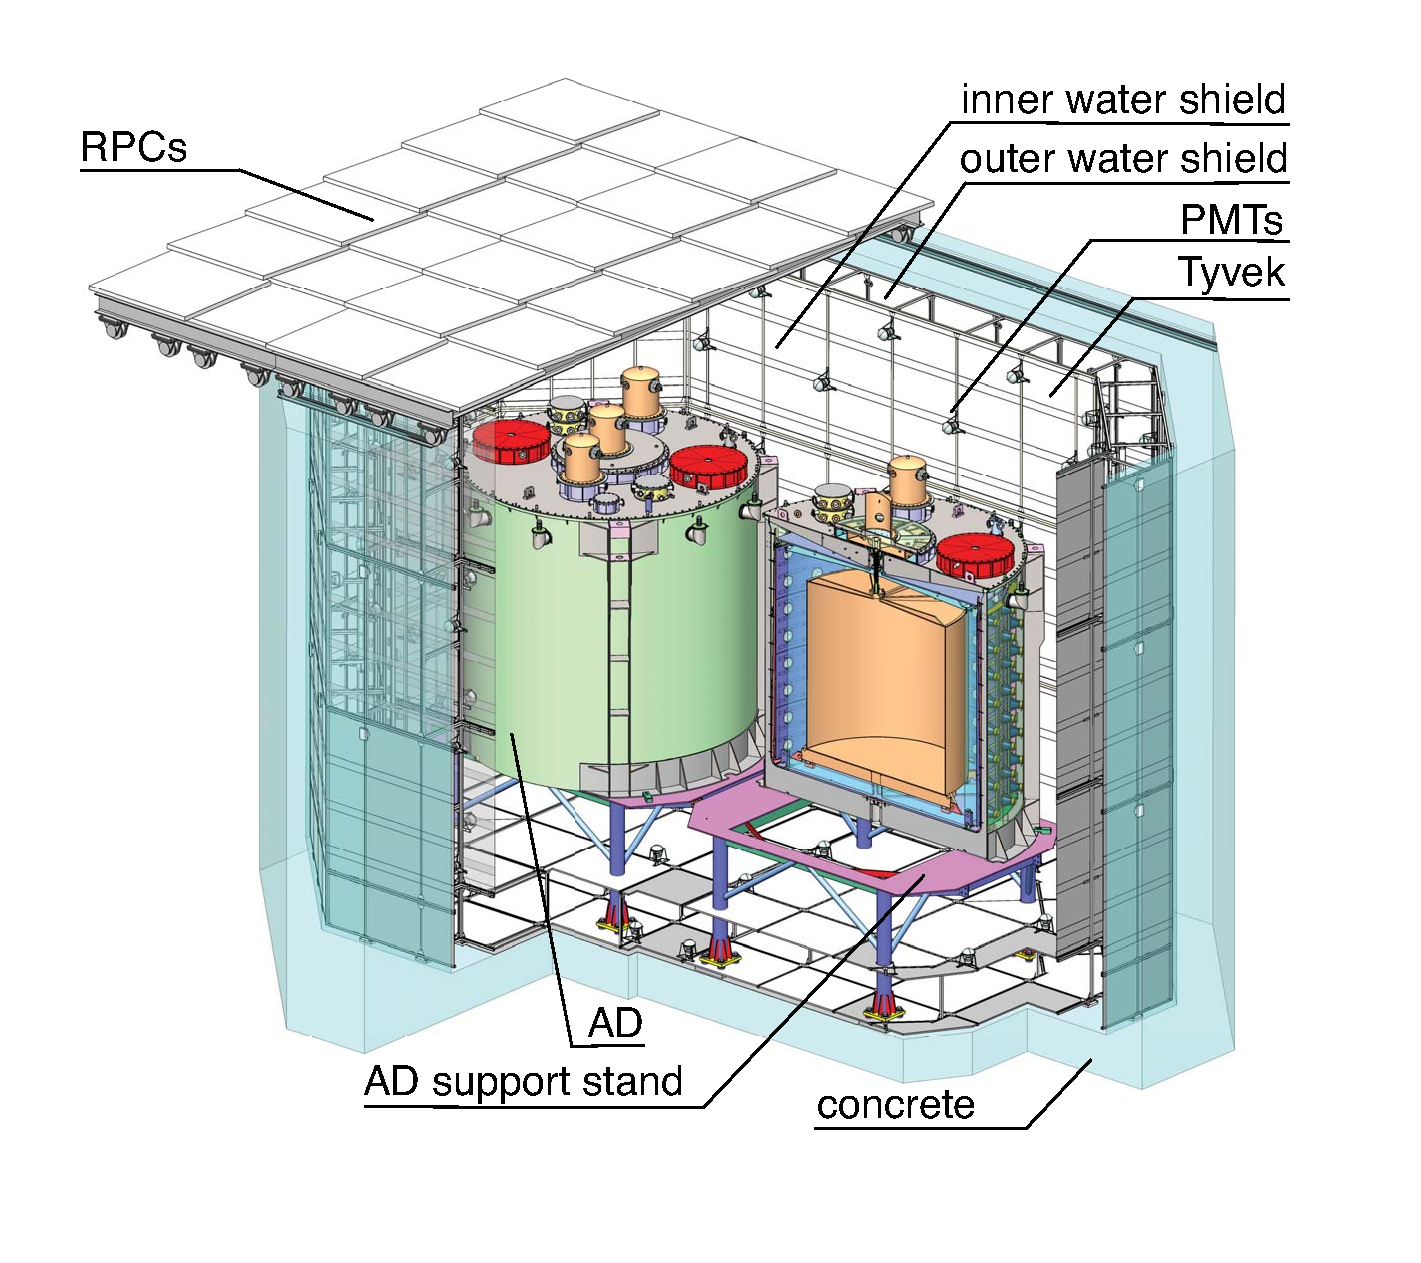
\includegraphics[height=0.4\textheight]{ch_detector/nearSiteDiagram}
    \caption{The water pool and AD layout in the near halls EH1 and EH2}
    \label{fig:wpcutout}
\end{figure}



\section{Triggers and data acquisition}

Each Daya Bay AD PMT has a single high-voltage (HV) coaxial cable
that supplies power to the PMT and returns the PMT signal to the
front-end electronics.
These electronics immediately start a TDC with \SI{1.6}{\ns} resolution,
and also measure the charge using a \SI{40}{\MHz} \num{12}-bit ADC
providing better than \num{0.1}-photoelectron (PE) resolution.
A \SI{50}{\percent} attenuated copy of the signal is passed to a copy
of the same ADC to allow for higher dynamic range in processing high-energy
events.
Refer to \cite[Sec.~II]{ngd2016} for the details
of the front-end electronics system.
The threshold to activate a single PMT channel's front-end electronics
is approximately \SI{0.25}{\pe}.
Once a channel is activated, the ADC values are buffered
awaiting a full-detector trigger signal.

The various detectors in an EH are triggered independently
by a master trigger board based on the conditions given in \cref{tab:trigger}.
Note that the trigger criteria are lower than the event selection
criteria used for the \thetaot{} analysis and described in \cref{ch:event_selection}.
Each channel's TDC is stopped when it receives a trigger signal
from the master trigger board.
For every channel with a TDC reading of \SI{<1.2}{\us},
the TDC reading, peak ADC value and the pedestal ADC value
(the ADC output given no PMT signal)
are recorded into the offline storage system.
The absolute timestamp of the event is determined by a GPS-based clock
with \SI{25}{\ns} resolution and is also stored.
The resulting data files comprise the raw data from Daya Bay.


\begin{table}[ht]
    \centering
    \begin{tabular}[t]{lllp{6cm}}
        \hline
        Detector & Criterion & Threshold value ($\geq$) & Explanation\\
        \hline
        AD & NHIT & \num{45} & Number of PMTs over threshold \\
        AD & ESUM & $\SI{65}{\pe}\approx \SI{0.4}{\MeV}$ & Analog sum of signals \\
        IWS & NHIT & \num{6} & \\
        OWS (near-hall) & NHIT & \num{7} & \\
        OWS (far-hall) & NHIT & \num{8} & \\
        AD & CALIB & - & Calibration trigger simultaneous with LED flash \\
        \hline
        \multicolumn{4}{c}{Ignored triggers for \thetaot{} analysis} \\
                       \hline
        RPC & NHIT & \num{3} & Number of layers over threshold in a single module \\
        AD & RANDOM & - & Random triggers issued at \SI{10}{\Hz} \\
        All & XTRIG & - & Criteria at one detector can trigger another \\
        \hline
    \end{tabular}
    \caption{Trigger criteria from \cite{ngd2016}}
    \label{tab:trigger}
\end{table}


\section{Previous results}

Since the start of data taking on 24 December 2011,
the Daya Bay experiment has produced numerous measurements of
\thetaot{}, (searches for) sterile neutrinos, reactor \nuebar{} flux,
and a variety of other physical phenomena.
The first Daya Bay measurement of \thetaot{} in April 2012
was the first nonzero measurement of that quantity.
This measurement used \SI{55}{\day} of \nuebar{} data
and, as mentioned previously, only six ADs were operational at the time.
Since then, Daya Bay has published updated results using IBDs detected by
either neutron capture on Gadolinium (nGd)
(\cite{ngd2012,ngd2013,ngd2014,ngd2015,ngd2016,ngd2018}) or neutron capture on Hydrogen (nH),
as shown in \cref{fig:theta13_vs_t}.

\begin{figure}
    \centering
    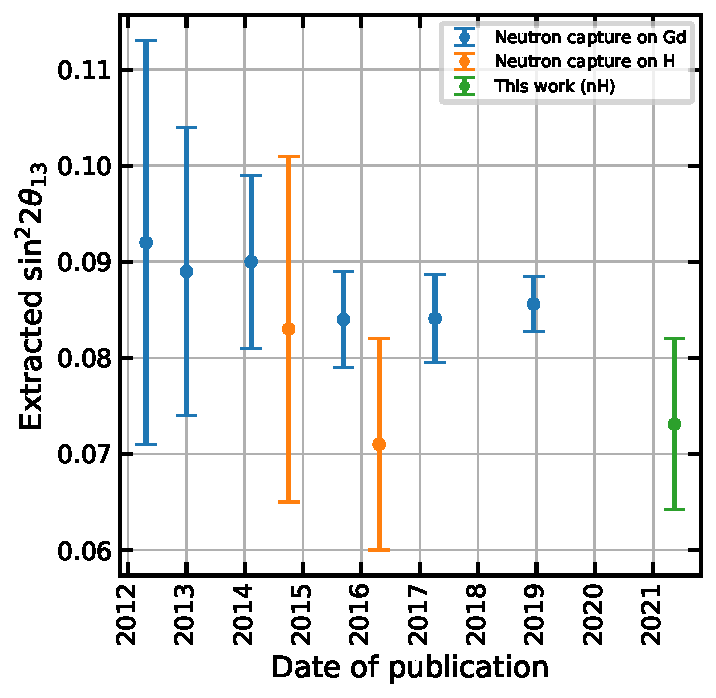
\includegraphics[height=0.4\textheight]{ch_detector/theta13_vs_time}
    \caption{
        Published values of $\sin^{2}2\thetaot$ over time
        for both nGd and nH analyses.
        Some nGd results are presented with separate statistical
        and systematic errors;
        those have been combined linearly for this plot.
    }
    \label{fig:theta13_vs_t}
\end{figure}

